% 
% Annual Cognitive Science Conference
% Sample LaTeX Paper -- Proceedings Format
% 

% Original : Ashwin Ram (ashwin@cc.gatech.edu)       04/01/1994
% Modified : Johanna Moore (jmoore@cs.pitt.edu)      03/17/1995
% Modified : David Noelle (noelle@ucsd.edu)          03/15/1996
% Modified : Pat Langley (langley@cs.stanford.edu)   01/26/1997
% Latex2e corrections by Ramin Charles Nakisa        01/28/1997 
% Modified : Tina Eliassi-Rad (eliassi@cs.wisc.edu)  01/31/1998
% Modified : Trisha Yannuzzi (trisha@ircs.upenn.edu) 12/28/1999 (in process)
% Modified : Mary Ellen Foster (M.E.Foster@ed.ac.uk) 12/11/2000
% Modified : Ken Forbus                              01/23/2004
% Modified : Eli M. Silk (esilk@pitt.edu)            05/24/2005
% Modified : Niels Taatgen (taatgen@cmu.edu)         10/24/2006
% Modified : David Noelle (dnoelle@ucmerced.edu)     11/19/2014

%% Change "letterpaper" in the following line to "a4paper" if you must.

\documentclass[10pt,letterpaper]{article}

\usepackage{cogsci}
\usepackage{pslatex}
\usepackage{apacite}
\usepackage{graphicx}
\usepackage{amssymb,amsfonts,amsmath}
\usepackage{todonotes}

\title{Let's talk (ironically) about the weather: A computational model of verbal irony}
 
\author{{\large \bf Justine T. Kao
(justinek@stanford.edu)} \\
  Department of Psychology, 450 Serra Mall \\
  Stanford, CA 94305 USA
  \AND {\large \bf Noah D. Goodman (ngoodman@stanford.edu)} \\
  Department of Psychology, 450 Serra Mall \\
  Stanford, CA 94305 USA}


\begin{document}

\maketitle


\begin{abstract}
Verbal irony plays an important role in how we communicate and express our opinions about the world. While there exist many interesting theories and empirical findings about how people use and understand verbal irony, there is to our knowledge no formal model of how people incorporate shared background knowledge and linguistic information to communicate ironically. Here we present two behavioral experiments that examine people's interpretations of utterances given different contexts in the weather domain. We then describe a computational model that reasons about background knowledge, affect, and the speaker's communicate goals to interpret ironic utterances and their rich affective subtexts. We show that by accounting for two types of affect goals---valence and arousal---our model produces interpretations that closely match humans'. Finally, we discuss the implications of our model on irony and its relationship to other types of nonliteral language understanding.


\textbf{Keywords:} 
irony; computational modeling; pragmatics; nonliteral language understanding
\end{abstract}


\section{Introduction}
\todo[inline]{RDH: Intro is great! Highly readable and makes the point of the paper very clear, even though I'm not super familiar with the literature on irony}
For better or for worse, verbal irony---roughly defined as utterances whose apparent meanings are opposite to the speaker's intended meaning \cite{roberts1994people, colston2000contrast}---is a major figurative trope of our time. From popular sitcoms to political satire to \emph{\#sarcasm} on Twitter and casual conversations among friends, verbal irony plays an important role in how we communicate and express  opinions about the world. The prevalence of verbal irony poses a puzzle for theories of language understanding: Why would speakers ever use an utterance to communicate its opposite meaning, and how can listeners appropriately interpret such an utterance? Previous work has shown that verbal irony serves several important communicative goals, such as to heighten or soften criticism \cite{colston1997salting}, elicit emotional reactions \cite{leggitt2000emotional}, highlight group membership \cite{gibbs2000irony}, and express affective attitudes \cite{colston1998you, colston1997ve}. These findings suggest that while ironic statements are false under their literal meanings, they are often highly informative with respect to social and affective meanings. 
In this paper, we present a computational model and behavioral experiments to show that people may use inferences about these alternative dimensions of meaning and the speaker's communicative goals to understand ironic utterances.  

\todo[inline]{RDH: maybe say \emph{which} alternative dimensions of meaning you'll be focusing on, to set up the distinction you make with the hyperbole model later? Right now, it looks like `alternative' means `social and affective,' but that's not exactly the set of dimensions you use later, right?}

Linguists and psychologists have proposed several informal theories of how people understand verbal irony. According to a classic Grician analysis, listeners first need to recognize that an ironic utterance blatantly violates the maxim of quality (to be truthful); they then arrive at a conversational implicature that the intended meaning is contrary to the utterance's literal meaning \cite{grice20134, wilson2006pragmatics}. While Grice's account is appealing in its treatment of verbal irony as arising naturally from conversational maxims, it does not provide a detailed or satisfactory explanation for how the appropriate implicature is derived from these maxims \cite{wilson2006pragmatics} 
\todo[inline] {RDH: Maybe give a quick, succinct reason this fails? I don't see the problem\dots but maybe it's not worth the space and I should just read the Wilson paper ;)}
On the other hand, previous work suggests that it is possible and indeed desirable to consider figurative language understanding as a product of general principals of communication, such as reasoning about informativeness with respect to the speaker's communicative goals \cite{kao2014nonliteral, kao2014formalizing}. In particular, a model that reasons about the speaker's affective goals is able to interpret hyperbolic utterances and infer the appropriate affective subtext \cite{kao2014nonliteral}. Given the fact that many researchers believe hyperbole and irony to be closely related phenomena (cite), we suggest that similar principles may account for verbal irony understanding as well. Our goal in this paper is to identify these communicative principles and provide a precise formal account of how they interact to produce ironic interpretations.

\begin{figure*}
\begin{minipage}{0.5\textwidth}
\scalebox{0.4}{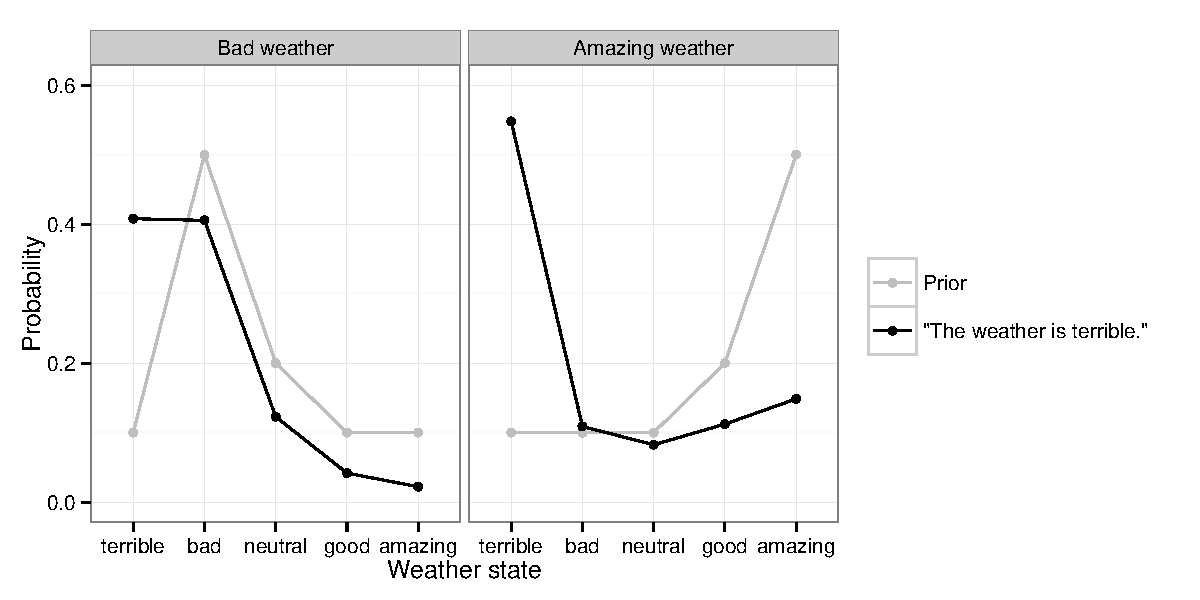
\includegraphics{simulation-1affect}}
\caption{Model interpretations of the utterance ``The weather is terrible" for different prior beliefs about the weather state given one affect variable: emotional valence. Gray lines indicate prior beliefs about weather states; black lines indicate posterior beliefs about weather states given the utterance.}
\label{sim1}
\end{minipage}
\begin{minipage}{0.5\textwidth}
\scalebox{0.4}{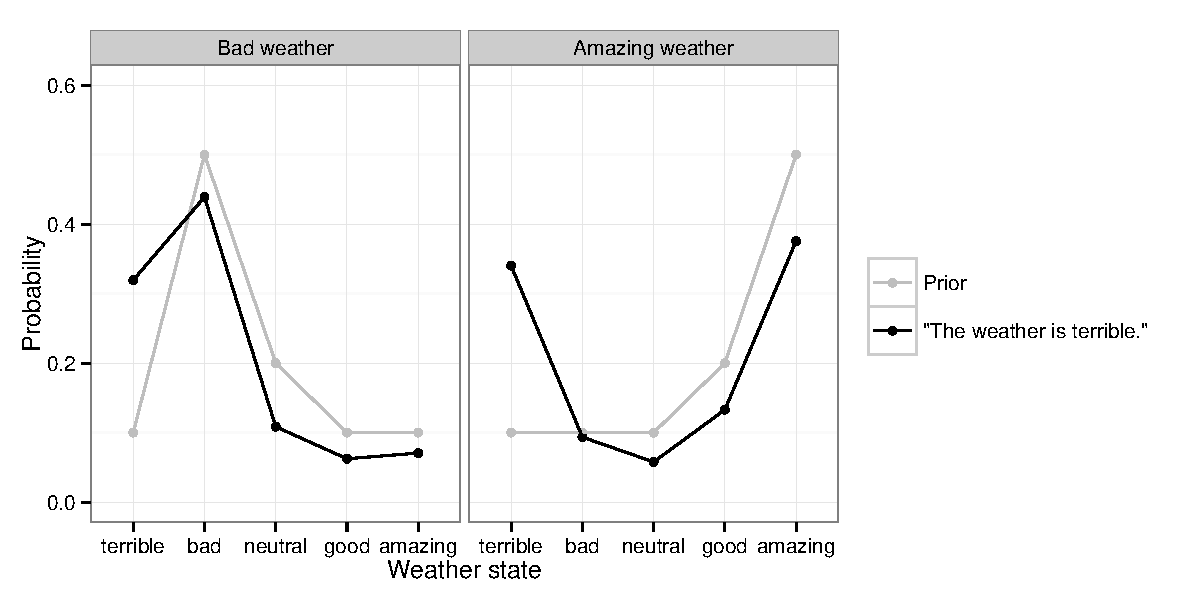
\includegraphics{simulation-2affect}}
\caption{Model interpretations for different prior beliefs about the weather state given two affect variables: emotional valence and emotional arousal. Gray lines indicate prior beliefs about weather states; black lines indicate posterior beliefs about weather states given the utterance.}
\label{sim2}
\end{minipage}
\end{figure*}

Rational Speech Act (RSA) models are a family of computational models that formalize language understanding as recursive reasoning between speaker and listener, and have been shown to account for many phenomena in pragmatics \cite{frank2012predicting, goodman2013knowledge}. \cite{kao2014nonliteral} introduces a critical extension to basic RSA models by considering the idea that speakers may aim to address different questions under discussion (QUDs) when formulating an utterance. An important task for the listener is to then jointly infer the QUD as well as the speaker's intended meaning. For example, a speaker may want to communicate negative affect about a situation (e.g. unhappiness about the temperature outside) instead of the precise situation (e.g. the precise temperature outside), in which case choosing an exaggerated utterance (e.g. ``It's freezing outside!") effectively addresses the QUD. A listener who reasons about the speaker and QUD is then able to use his background knowledge about temperatures to correctly infer that the speaker is upset about the temperature, but that it is unlikely to be literally freezing outside (especially if she is in California). Such a model extended to consider QUDs---which we will refer to as qRSA---opens up the possibility for a speaker to produce an utterance that is literally false but satisfies her goal to convey affect. While this model produces nonliteral interpretations of hyperbolic utterances that closely match humans', \cite{kao2014nonliteral} considered only a fairly impoverished space of affects, namely the presence or absence of negative feeling. This overlooks the range of attitudes and emotions that speakers could express with nonliteral utterances. In particular, since verbal irony involves expressing negative meanings with positive utterances and vice versa, a richer space of affect that includes both positive and negative emotions is necessary. Here we examine the consequence of considering a range of emotions in an empirically derived two-dimensional affect space within the qRSA model, and show that this minimal change is able to capture verbal irony.


%Here we present a computational model that takes into account common ground and affective dimensions of meaning to model how people understand irony. 

%Since Grice's original proposal, there have been two competing theories of irony understanding: the echoic mention theory \cite{sperber1981irony, jorgensen1984test} and pretense theory \cite{clark1984pretense}. Both theories move away from a straightforward framework of pragmatics. While these informal theories each offer interesting insights into certain aspects of irony, determining which particular theory is superior is beyond the scope of this paper. Instead, we are interested in identifying basic elements of irony that are consistent across different theoretical frameworks and providing a precise formal account of how these elements can be incorporated to produce ironic interpretations. 



%While there are interesting theories and empirical findings about how people use and understand verbal irony, there is to our knowledge no formal model of how people incorporate shared background knowledge and linguistic information to communicate about the world and their attitudes using irony. 

%We observe that across different approaches to verbal irony, researchers agree that common ground between speaker and listener is critical for successful interpretation \cite{williams1984does}. In addition, verbal irony almost always communicates the speaker's attitude about a certain topic (cite). 



In what follows, we will examine interpretations of potentially ironic utterances in an innocuous domain---the weather. We chose the weather as the victim of irony for several reasons. First, people are quite familiar with talking (and complaining) about the weather. Second, we can visually represent the weather to participants with minimal linguistic description in order to obtain measures of nonlinguistic contextual knowledge. Finally, we can vary the weather states to observe how the same utterance is interpreted differently given different contextual knowledges. We first describe an extension to the qRSA model and show that an enriched space of affect enables the model to produce ironic interpretations. We then present two behavioral experiments that examine people's interpretations of utterances given different weather contexts. We show that by accounting for two types of affect goals, valence and arousal, our model produces interpretations that closely match humans'. Finally, we discuss the implications of our model on irony and its relationship to other types of nonliteral language understanding.


\section{Computational Model}
%Our behavioral experiments confirmed that people's judgments of irony are highly sensitive to their prior knowledge of the world. We also showed that two affective dimensions---valence and arousal---may be especially important for irony. Here we describe an extension to the basic Rational Speech Act (RSA) model that incorporates these elements to produce interpretations of ironic utterances. 


%
%The extended model was able to produce appropriate interpretations of hyperbole as well as its affective subtext. However, since the model only considered a fairly impoverished affect goal (communicating presence or absence of negative affect), it could not take into account cases where a negative utterance is used to communicate positive affect (and vice versa), which is critical in ironic uses (e.g. saying ``Life is so hard!" when sipping iced lemonade on a sunny beach). 
%

In this section, we describe the qRSA model and compare its interpretations of utterances using one versus two dimensions of affect. 
%
%We begin with a literal listener $L_0$, who interprets all utterances literally. For example, the literal listener will interpret the utterance ``The weather is terrible" to mean that the weather state is \emph{terrible}, and that the speaker has the corresponding negative valence towards the weather. 
%
%Formally, if $u$ is the uttered adjective:
%\[ L_0(s, v, a|u) = \left\{ 
%  \begin{array}{l l}
%    P(v, a | s) & \quad \text{if $s$ = $u$}\\
%    0 & \quad \text{otherwise}
%  \end{array} \right.\]
%where $P(v, a | s)$ is the prior probability that a speaker would feel valence $v$ and arousal $a$ towards the weather state $s$.
%
%We assume that the speaker's goal $g$ is to communicate  along any (or multiple) of the three dimensions of meaning, which results in $2^3 - 1 = 7$ possible goals (the speaker cannot communicate along none of the dimensions). For example, the speaker may want to communicate only the weather state $s$, or only her valence about $s$, or both.
%We assume that the QUD may be about the actual weather, or the speaker's emotional valence towards the weather. 
Following the qRSA model described in \cite{kao2014nonliteral}, a speaker chooses an utterance that most effectively communicates information regarding the question under discussion (QUD) to a literal listener, where the QUD can be the state of the world $s$ or the speaker's affect towards the state, $a$.
We define the speaker's utility as the negative surprisal of the true state under the listener's distribution given an utterance; however, since a QUD is a projection from the full meaning space to the subset of interest to the speaker, we consider only surprisal along the QUD dimension.   
\todo[inline]{RDH: 1. maybe write out this utility function mathematically? 2. what is the meaning space? Is this just the world space? Or the set of features indexing the world space? 3. maybe explain what the subscripts mean? Using a subscript for $S_1$ sets it up for there to be an $S_2$ or $S_0$, which there isn't!}
%This leads to the following utility function for speaker $S_1$:
%\begin{equation}
%U(u | s, v, a, g) = \log \sum_{s', v', a'} \delta_{g(s, v, a)=g(s', v', a')} L_0(s, v, a |u)
%\end{equation}
Given this utility function, the speaker chooses an utterance according to a softmax decision rule \cite{sutton1998reinforcement}\footnote{See \cite{kao2014nonliteral} for details}:
\begin{equation}
S_1(u | s, a, q) \propto e^{\lambda U(u | s, a, q)},
\end{equation}
where $q$ is the QUD and $\lambda$ is an optimality parameter.
%
Imagine that $S_1$ has the goal to convey negative feelings towards the weather. Based on $S_1$'s understanding of $L_0$'s prior knowledge, she knows that if she produces the utterance ``The weather is terrible," $L_0$ will believe that the weather is terrible and that the speaker is likely to feel negative about it. Since the QUD is successfully addressed if the listener believes that $S_1$ feels negative towards the weather state, $S_1$ is motivated to produce such an utterance.  A pragmatic listener $L_1$, on the other hand, takes into account prior knowledge and his internal model of the speaker to determine the intended meaning. Because $L_1$ is uncertain about the QUD, he marginalizes over the possible QUDs under consideration:
$$
L_1 (s, a | u) \propto P(s) P(a | s) \sum_{q}{P (q) S_1 (u|s, a, q)}
$$
%
\todo[inline]{RDH: It might be helpful here to point out that you're going to try different ways of specifying the QUD space. Otherwise, it may not be clear what you're `considering' these spaces for.}
We first consider a simple affect space, which we call $a_1$: whether the speaker feels negative or positive about $s$. This is essentially equivalent to the hyperbole model described in \cite{kao2014nonliteral}, except the binary affect variable $v$ can take on the values \emph{positive} and \emph{negative} instead of \emph{negative} and \emph{not-negative}.
%
%If $L_1$ thinks it is likely that speaker $S_1$'s goal is to convey negative emotion but believes that it is \emph{a priori} unlikely for the weather state to be \emph{terrible}, he will determine that $S_1$ feels negative about the weather, but that the weather state is more likely less extreme than \emph{terrible}. This produces a hyperbolic interpretation of the utterance. However, if $L_1$ thinks it is \emph{a priori} extremely likely for the weather state to be \emph{amazing}, upon hearing ``The weather is terrible," he will believe that the weather is terrible, because otherwise there is no reason for $S_1$ to choose that utterance. In other words, this model cannot infer a positive state from a negative utterance (and vice versa), thus failing on most cases of verbal irony. 
%
Figure~\ref{sim1} shows simulations of this model with a simple one-dimensional affect space. Given strong prior belief that the weather state is \emph{bad}, the model interprets the utterance ``The weather is terrible" to mean that the weather is equally likely to be \emph{terrible} or \emph{bad}, producing a hyperbolic interpretation of the utterance. However, given strong prior belief that the weather is \emph{amazing}, the model interprets the utterance ``The weather is terrible" to mean that the weather is indeed terrible, because otherwise there is no reason for the speaker to choose that utterance. In other words, this model cannot infer a positive state from a negative utterance (and vice versa), thus failing on most cases of verbal irony. 

\todo[inline]{JTK: rework writing}
We now consider a more complex affect space ($a2$) to observe its consequence on interpretation. Affective science identifies valence and arousal as two main dimensions underlying the slew of emotions people experience (cite). Valence and arousal are found to be quadratically related, with strong negative valence and strong positive valence associated with high arousal. Speakers may leverage this relationship between valence and arousal to convey high arousal and positive affect using strong negative utterances. Figure~\ref{sim2} shows simulations of the qRSA model with a  two-dimensional affect space, valence and arousal. Given strong prior belief that the weather state is \emph{bad}, the model interprets ``The weather is terrible" to mean that the weather is likely to be \emph{bad}, producing a hyperbolic interpretation. However, given strong prior belief that the weather is \emph{amazing}, the model now interprets ``The weather is terrible" to mean that the weather is likely amazing. This suggests that reasoning about a richer two-dimensional affect space may enable the model to appropriately interpret ironic utterances. 

\todo[inline]{RDH: maybe clarify the distinction between these spaces a bit -- is $a_2$ arousal + valence, while $a_1$ is just valence? It seems counterintuitive that adding \emph{arousal} would give rise to these effects... And not necessarily predicted by previous work?}
%\todo[inline]{JTK: But do we refer to these affect dimensions as valence and arousal? Without first introducing these dimensions with the experiment, how should we talk about them in the model?}

%\todo[inline]{let's try to compress this formal model description, given that it is the same as the PNAS paper. perhaps just say that we give a sketch, and the details can be found in the other paper?}

\section{Behavioral Experiments}
We conducted the following two experiments to test our model with the enriched affect space described above. In Experiment 1, we measured the prior beliefs over weather states for various contexts as well as the relevant affect dimensions. In Experiment 2, we collected people's ratings of a speaker's judgment of and feelings towards the weather given what she says about it (e.g. ``The weather is terrible!" when the context clearly depicts sunny weather).

%\todo[inline]{I would emphasize in motivating this that we want to explore how the true affective response space can explain irony. Hence we measure the state priors but also measure a bunch of dimensions of potential variance of affect. We can then do dimensionality reduction to extract the true affective dimensions to construct an affect-given-state prior. In model comparison below, make sure we test keeping different numbers of components from the PCA.

%Also make it more clear that the reason to do these experiments is to test a theory of irony understanding, to be described later, that depends on this background knowledge. Maybe the model should go first?}

%We conducted the following two experiments to elicit people's judgements of potentially ironic utterances and their relationship to context and background knowledge. In Experiment 1, we collected participants' ratings of various weather contexts as well as how a person (e.g. Ann) feels about the weather. The weather ratings measure knowledge of the current weather state. The affect ratings measure how people generally feel about different weather states, which captures people's intuitive theory of attitudes towards the weather. In Experiment 2, we collected people's ratings of Ann's judgment of and feelings towards the weather given what she says about it, for example, ``The weather is terrible!" when the weather depicted is clearly sunny and nice.

\subsection{Experiment 1: Prior elicitation}
\subsubsection{Materials and methods}
We selected nine images from Google Images that depict the weather. To cover a range of weather states, three of the images were of sunny weather, three of cloudy weather, and three of rainy or snowy weather. Each of these images represents a \emph{weather context}, or $w_i$. The images can be found here: \todo[inline]{RDH: would you want to put this grid in a figure?}

$49$ native English speakers with IP addresses in the United States were recruited on Amazon's Mechanical Turk. Each participant saw all nine images in random order. In each trial, participants were told that a person (e.g. Ann) looks out the window and sees the view depicted by the image. They then indicated how Ann would rate the weather using a labeled 5-point Likert scale, ranging from \emph{terrible}, \emph{bad}, \emph{neutral}, \emph{good}, to \emph{amazing}. Finally, participants used slider bars to rate how likely Ann is to feel each of the following seven emotions about the weather: \emph{excited}, \emph{happy}, \emph{content}, \emph{neutral}, \emph{sad}, \emph{disgusted}, and \emph{angry}. \todo{why these seven? basic emotions according to someone?} The order of the emotions were randomized for each participant but remained consistent across trials for the same participant. The end points of the slider bars were labeled as ``Impossible" and ``Absolutely certain." A link to the experiment is here:
  
\subsubsection{Results}
\begin{figure}[t]
\scalebox{0.4}{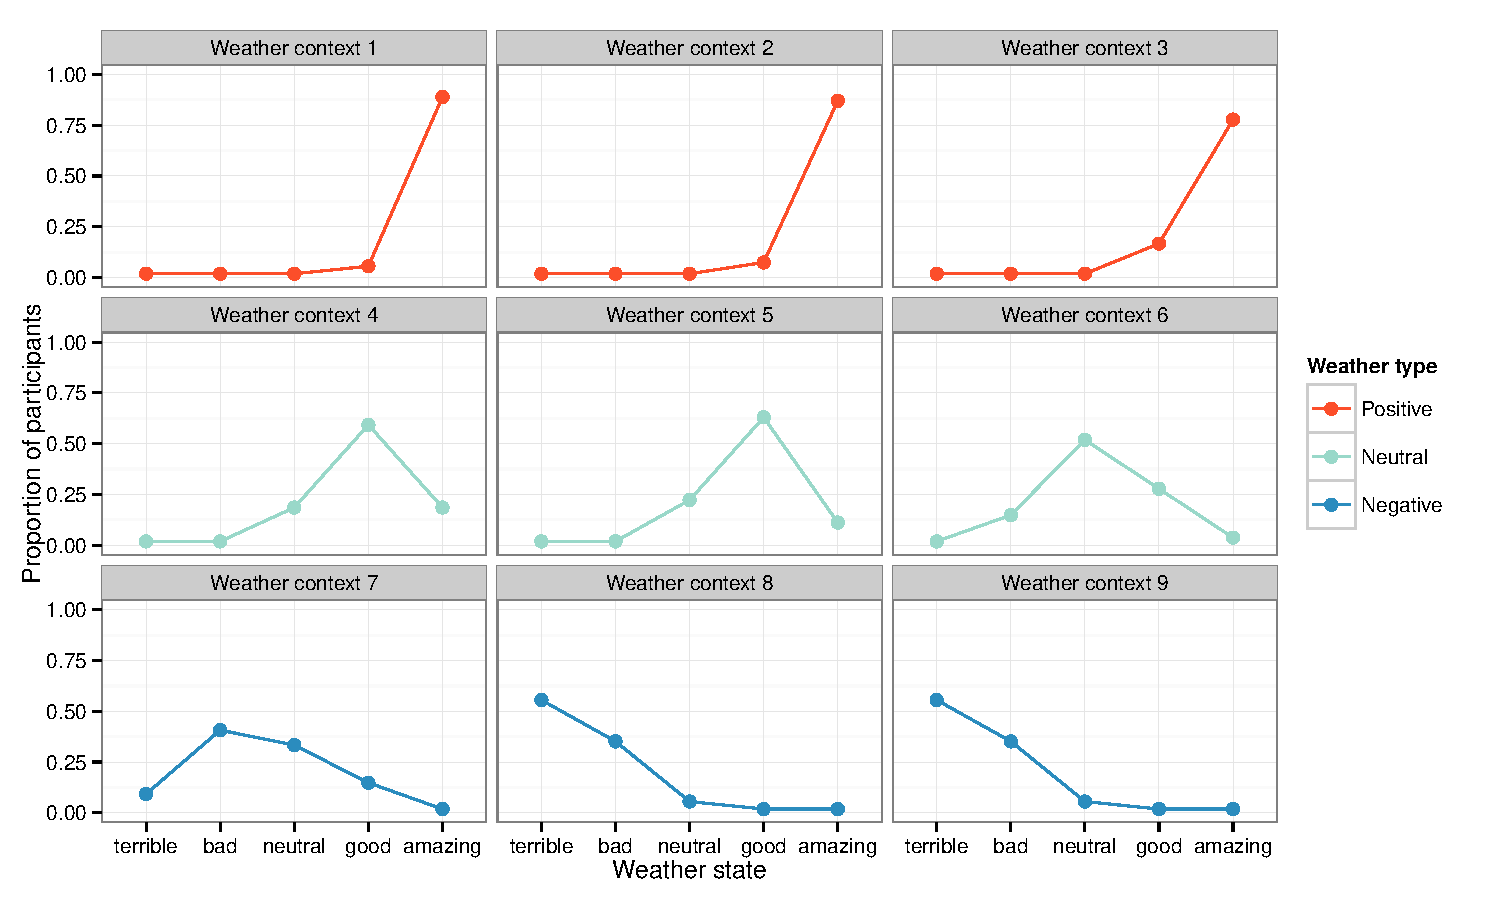
\includegraphics{priors.pdf}}
\caption{The proportion of participants who rated each of the weather contexts ($w_i$) as each weather state. Each panel represents a weather context; each line represents the distribution over weather states for a weather context prior to any linguistic input. For example, the vast majority of participants rated $w_1$ as \emph{amazing}, suggesting that the prior probability of someone believing $w_1$ to be \emph{amazing} is extremely high.}
\label{priors}
\end{figure}

\begin{figure*}
\begin{minipage}{0.5\textwidth}
\scalebox{0.5}{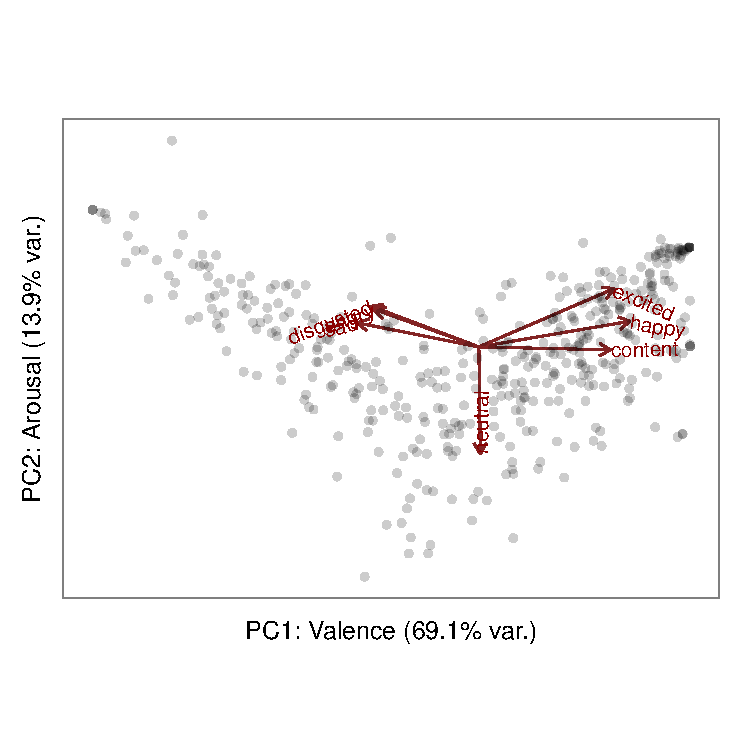
\includegraphics{biplot.pdf}}
\caption{A biplot of the two principal components of the emotion ratings from Experiment 1. PC1 corresponds roughly to positive valence, with higher values for \emph{content, happy}, and \emph{excited} and lower values for \emph{sad, angry}, and \emph{disgusted}. PC2 corresponds roughly to high arousal, with higher values for \emph{excited} and {disgusted} than for \emph{content} and \emph{neutral}.}
\label{PCA}
\end{minipage}
\begin{minipage}{0.5\textwidth}
\scalebox{0.6}{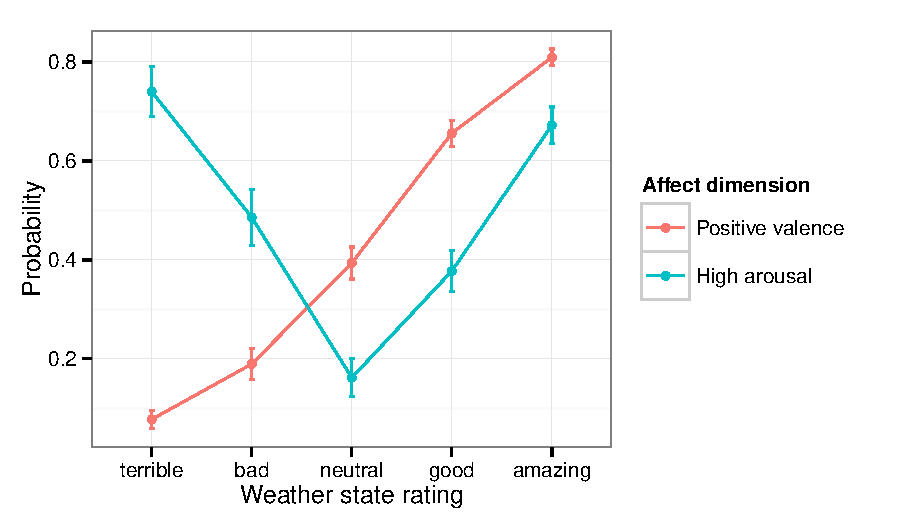
\includegraphics{affect-prior.pdf}}
\caption{The average probabilities of positive valence and high arousal associated with each weather state. Error bars are $95\%$ confidence intervals.}
\label{affect-prior}
\end{minipage}
\end{figure*}

For each of the nine weather contexts, we obtained the number of participants who gave each of the weather state ratings and performed add-one Laplace smoothing on the counts. This allowed us to compute a smoothed prior distribution over weather states given each context (see Figure ~\ref{priors}). \todo[inline]{RDH: obviously, need some way of identifying what the different rows and columns of the grid mean}
%
To examine participants' ratings of the affects associated with each context, we first performed Principal Component Analysis (PCA) on the seven emotion category ratings. This allowed us to compress the ratings onto a lower-dimensional space and also reveal the main affective dimensions that are important in this domain. We found that the first two principal components accounted for $69.14\%$ and $13.86\%$ of the variance in the data (see Figure ~\ref{PCA}). In addition, they correspond roughly to the dimensions of emotional valence (positive or negative) and emotional arousal (high or low), respectively, which are consistent with theories of emotion in affective science (cite). 
\todo{we should do a free response version of this task (``Ann feels ..... about the weather.''), before and after a statement, at some point to see if we are missing any affects... probably not needed for cogsci.}
In order to examine the probabilities of Ann feeling positive or negative affect and high or low arousal given different weather states, we converted the PCA scores into probabilities as follows. We first normalized the scores in each dimension to have zero mean and unit variance. Treating these normalized scores as quantiles of a standard normal distribution, we used the cumulative distribution function to convert the normalized scores into values between $0$ and $1$. 
\todo{JTK: something about how this is not a perfect transformation but does approximately the right thing} Figure ~\ref{affect-prior} shows the probability of positive valence and high arousal given each weather state.

%\begin{figure}
%\begin{minipage}[b]{.5\textwidth}
%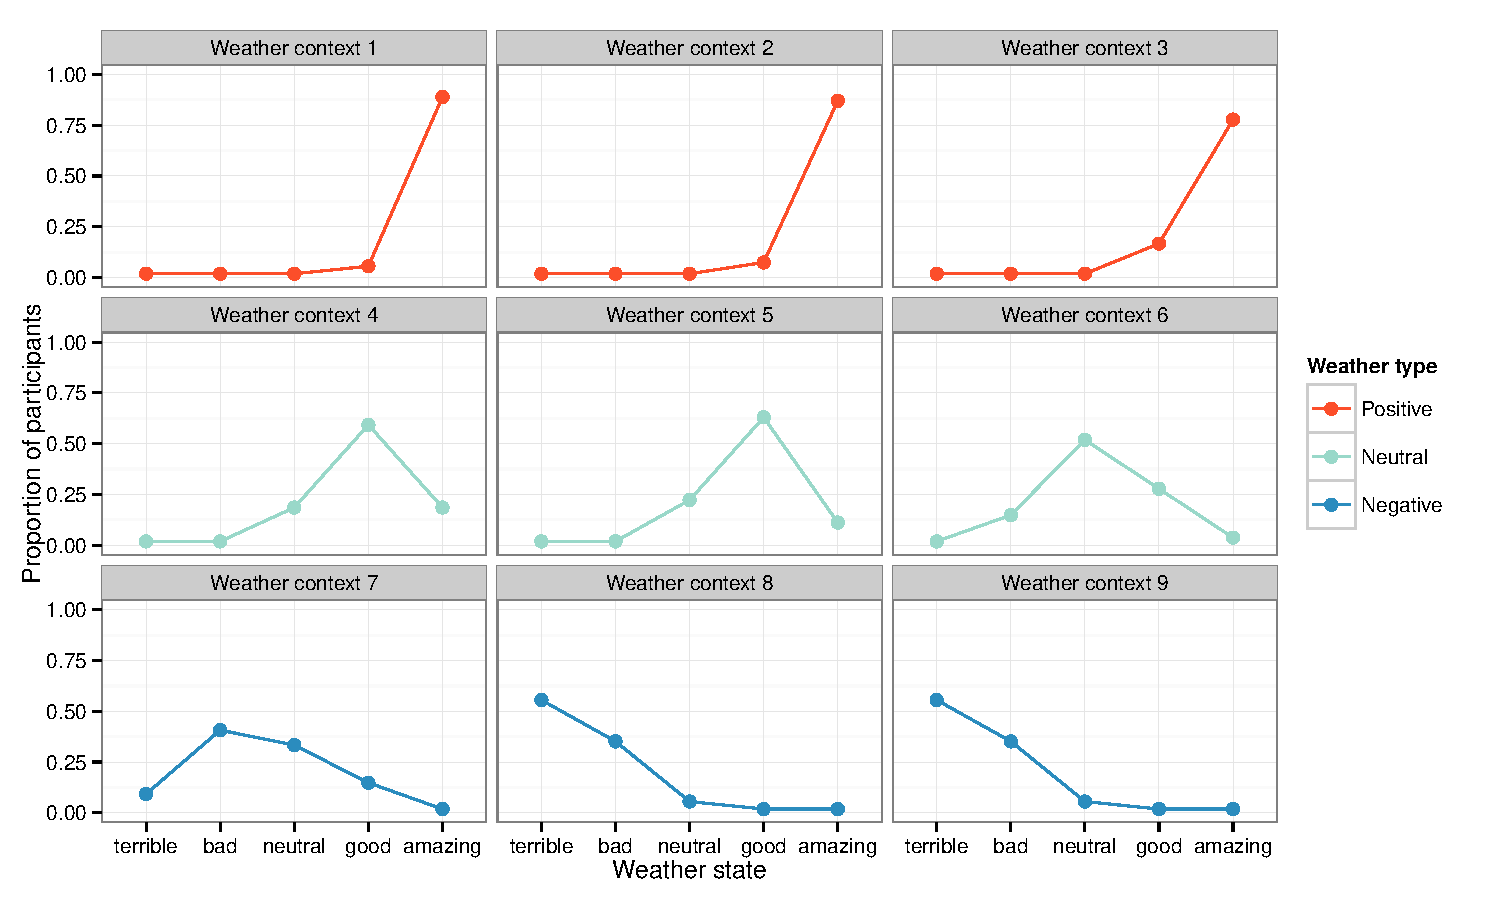
\includegraphics[width=5cm, height=3.7cm]{priors.pdf}
%\end{minipage}
%\begin{minipage}[b]{.4\textwidth}
%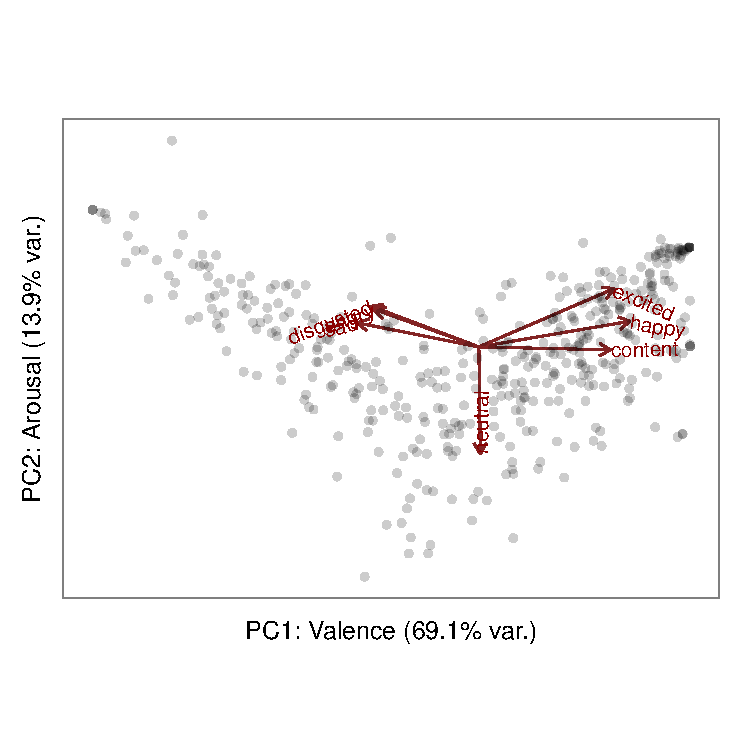
\includegraphics[width=5cm, height=5cm]{biplot.pdf}
%\end{minipage}
%
%\end{figure}

\subsection{Experiment 2: Irony understanding}
\subsubsection{Materials and methods}
We used the same nine weather images from Experiment 1. $59$ native English speakers with IP addresses in the United States were recruited on Amazon's Mechanical Turk. Each participant saw all nine images in random order. In each trial, participants were told that Ann (characters' names were randomized) and her friend look out the window together and sees the view depicted by the image. Ann says, ``The weather is \underline{\hspace{1cm}}!" where the adjective is randomly selected at each trial from the following set: ``terrible," ``bad," ``ok," ``good," and ``amazing." Participants first rated how likely it is that Ann's statement is ironic using a slider with end points labeled ``Definitely NOT ironic" and ``Definitely ironic." They then indicated how Ann would actually rate the weather using a labeled 5-point Likert scale, ranging from \emph{terrible}, \emph{bad}, \emph{neutral}, \emph{good}, to \emph{amazing}. Finally, participants used sliders to rate how likely it is that Ann feels each of the seven emotions about the weather. A link to the experiment is here:

\subsubsection{Results}
We first examined participants' irony ratings for each of the weather context and utterance pairs. We coded ``terrible" and ``bad" as \emph{negative} utterances, ``ok" as a \emph{neutral} utterance, and ``good" and ``amazing" as \emph{positive} utterances. We also coded each image as \emph{positive, neutral}, or \emph{negative} based on the modal weather state rating from Experiment 1 (e.g. $w_1$ is \emph{positive}, $w_6$ is \emph{neutral}, and $w7$ is \emph{negative}). We found a basic irony effect, where utterances whose polarities are inconsistent with the polarity of the weather context (e.g. using ``terrible" to describe $w_1$) are rated as significantly more ironic than utterances whose polarities are consistent with the weather context (e.g. using ``good" or ``amazing" to describe $w_1$) (STATS) (Figure XX?). Furthermore, a linear regression model with the polarity of the utterance, the polarity of the weather context, and their interaction as predictors of irony ratings produced an adjusted R-squared of 0.91, capturing most of the variance in the data. 
\todo[inline]{RDH: I'm getting confused about utterance polarity vs. weather state polarity (possibly since they take on the same values), and this confusion compounded over the next paragraphs where you present more measures. Maybe lay this out in a way that distinguishes them better? Even putting ``utterance polarity'' and ``context polarity'' in bold font or something might help.}

\begin{figure*}[t]
\begin{minipage}{0.5\textwidth}
\scalebox{0.45}{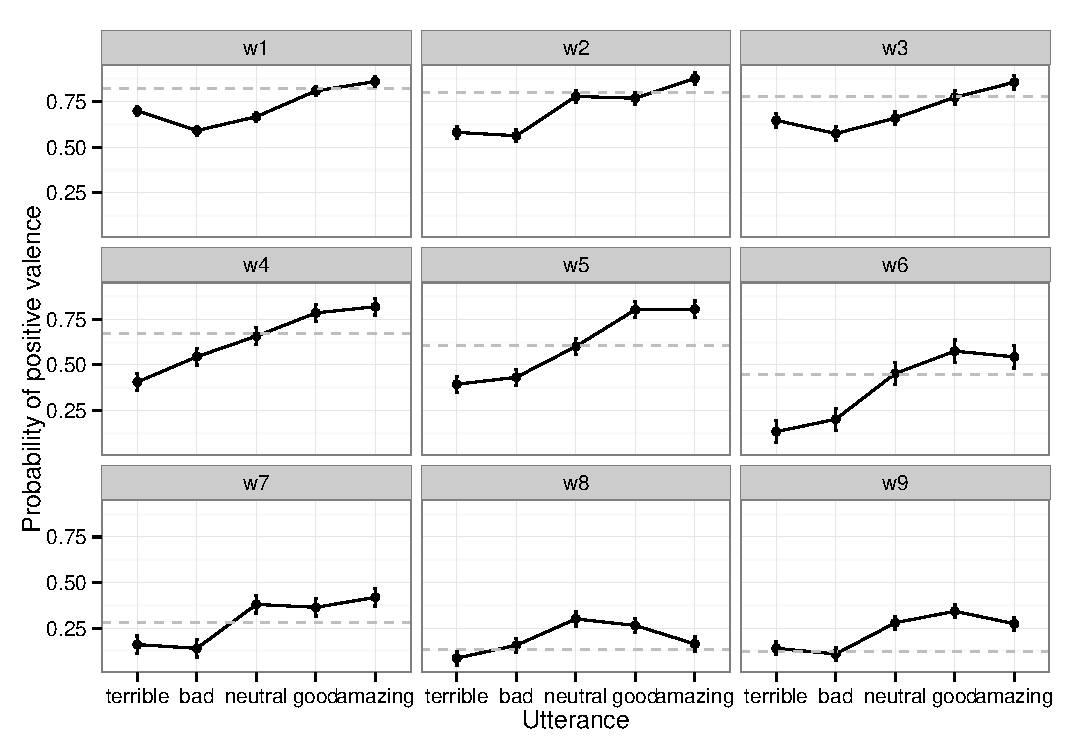
\includegraphics{valence.pdf}}
\caption{Average probabilities of the speaker feeling positive valence given her utterance about the weather context. Each panel represents a weather context ($w_i$). The dotted line is the prior positive valence associated with each weather context, taken from Experiment 1. The solid line represents the probability of positive valence given an utterance.}
\label{valence}
\end{minipage}
\begin{minipage}{0.5\textwidth}
\scalebox{0.45}{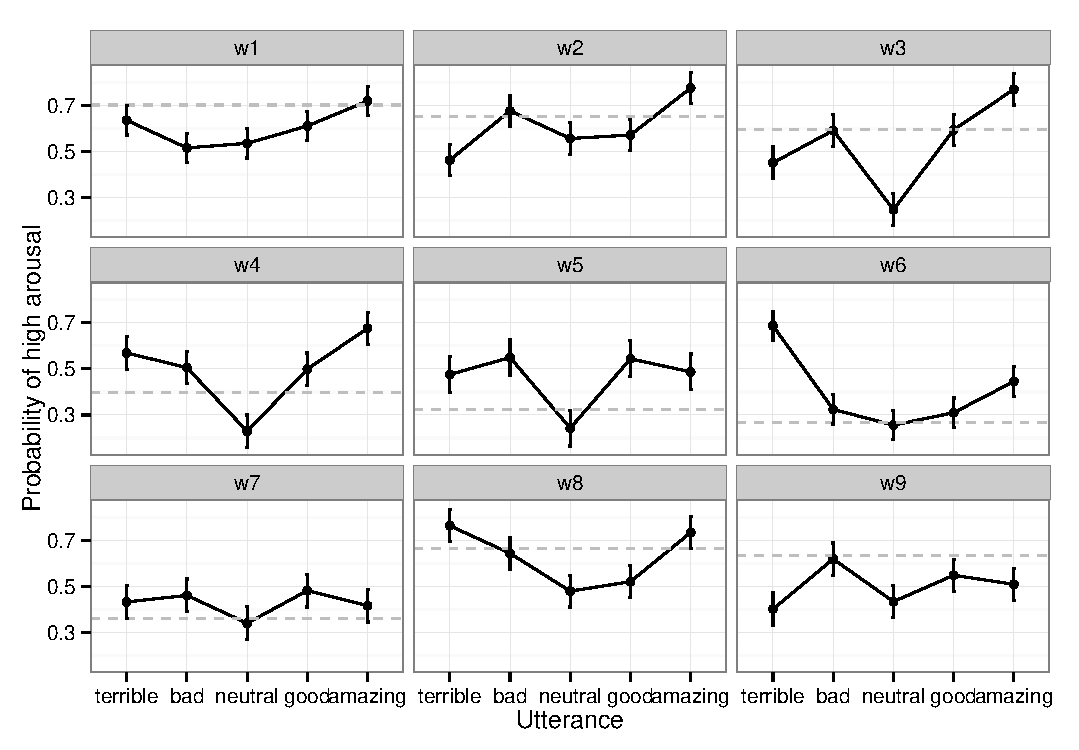
\includegraphics{arousal.pdf}}
\caption{Average probabilities of the speaker feeling high arousal given her utterance about a weather context. Each panel represents a weather context ($w_i$). The dotted line is the prior high arousal associated with each weather context, taken from Experiment 1. The solid line represents the probability of high arousal given an utterance.}
\label{arousal}
\end{minipage}
\end{figure*}

\todo[inline]{RDH: I don't quite understand what the KL divergence is measuring in the next paragraph}
We then examined participants' ratings of the weather context given an utterance. For each of the $45$ weather context (9) $\times$ utterance (5) pairs, we obtained the number of participants who gave each of the five weather ratings. After performing add-one Laplace smoothing on the counts, we computed a smoothed distribution over weather states given each context and utterance (Figure XX?). We call this distribution the \emph{interpreted meaning} of an utterance in context. We found that participants often rated the speaker (e.g. Ann) as judging the actual weather state to be different from what she described in her utterance, suggesting that participants interpreted these utterances non-literally. To further examine the relationship between literal meaning, interpreted meaning, and judgements of irony, we computed the Kullback-Leibler divergence between the literal interpretation of the utterance and the distribution over weather states given the context and utterance. 
\todo{what is the literal distribution? if it's delta on the word corresponding state, then isn't KL just the interpretation log-prob of the state?}
We found that adding the KL divergence measure to the linear regression model captured significantly more variance in the irony ratings, with an R-squared of 0.93 (more STATS). 
\todo{this doesn't seem like the right analysis.... and a 1\% gain is pretty minimal to fuss about.} 
This suggests that even beyond inconsistencies in polarity between utterance and context, people are sensitive to the fine-grained differences between literal and interpreted meanings in their judgements of irony.

Finally, we examined the emotions expressed by utterances in context. We used the loadings from the PCA on emotion ratings from Experiment 1 to predict the projected values of emotion ratings in Experiment 2 and performed the same transformations on the scores to convert them into values between $0$ and $1$. Figure ~\ref{valence} shows the average probability of positive valence given a weather context and an utterance. The dotted gray lines are the average probabilities of positive valence associated with each weather context without any linguistic input, taken from Experiment 1. We see that for the \emph{positive} weather contexts ($w_1, w_2, w_3$), the speaker is interpreted as more likely expressing positive valence given the extremely negative utterance ``terrible" than given the less negative utterance ``bad." On the other hand, for the \emph{negative} weather contexts ($w_7, w_8, w_9$), the speaker is interpreted as less likely expressing positive valence given the extremely positive utterance ``amazing than the less positive utterance ``good" (STATS). This suggests that extreme utterances that are inconsistent with the valence of the context are more likely to express an opposite affect than its literal meaning (MAKE THIS CLEARER).
\todo[inline]{maybe you could use different names for the weather contexts? Like $\mathcal{W}_{neg}, \mathcal{W}_{neut}, \mathcal{W}_{pos}$, and then refer to $w_i \in \mathcal{W}_{neg}$ and so on.}

Figure ~\ref{arousal} shows the average probability of high arousal given a weather context and an utterance. The dotted gray lines are the average probabilities of high arousal associated with each weather context without any linguistic input, taken from Experiment 1. We see that regardless of the weather context, more extreme utterances are more likely to express high arousal (MAKE THIS CLEARER). (Generally, just say that the utterance shifts interpreted valence and arousal away from the baseline). 
\todo{it's interesting that ``terrible'' seems to have suppressed arousal compared to ``bad''. any thoughts about why?}


\section{Model Evaluation}
In this section, we evaluate the model's performance using results from our behavioral experiments. To produce an interpretation of an utterance in context, the model requires the following input values: (1) the prior probability of a weather state $s$ for a given weather context, $P(s)$ (2) the joint probability of positive/negative valence given a weather state, $P(v, a | s)$ (3) the prior probability of a particular goal $P(g)$ (4) the speaker optimality parameter $\lambda$. We derived the values for (1) and (2) from Experiment 1 and fit (3) and (4) to the data from Experiment 2 (TODO: add actual fit values in a clear manner: $\lambda=1$, p(state goal) = 0.2, p(valence goal) = 0.3, p(arousal goal)=0.4).

The model produced an interpretation for each of the $45$ utterance $\times$ weather context pairs. Each interpretation is a joint posterior distribution $P(s, v, a | u)$. We first examine the model's performance on recovering the actual weather state $P(s | u)$ by marginalizing over $v$ and $a$. Figure ~\ref{model-state} shows participants' and the model's interpretation of the actual weather state given an utterance and a weather context. We see that the model predictions closely match humans' interpretations, with a correlation of $0.86$ (show scatter plot?). 
\todo{is the model using the prior too strongly here?}
Next, we examine the model's performance on recovering the speaker's valence by marginalizing over $s$ and $a$. The model's prediction for emotional valence match humans' extremely closely, with a correlation of $0.96$.
\todo{note that this is the case even when interpreted valence mismatches the prior expected valence given literal meaning -- i.e. the model captures irony in valence.}
Finally, we examine the model's performance on recovering the speaker's emotional arousal by marginalizing over $s$ and $v$. The model's prediction for emotional arousal match humans' with a correlation of $0.66$ (TODO: add split half; figures???). 
\todo{why is this correlation low? is it because of the terrible-bad inversion i asked about above?}
This suggests that the model is able to incorporate background knowledge and reasoning about multiple affective goals to produce the appropriate ironic interpretations as well as the associated affects. 
\todo{it would be nice to have some more direct analysis of irony -- that when state/valence mismatches that expected from literal meaning the model can predict it. this may also be a good place to come back to the explicit irony judgements: something like probability the interpretation is on the opposite side of the prior mean? or something more general that would also apply to ironic propositions? oh.. we should totally say something in the discussion about ironic propositions and other non-scalar irony.}


\begin{figure}[t]
\scalebox{0.5}{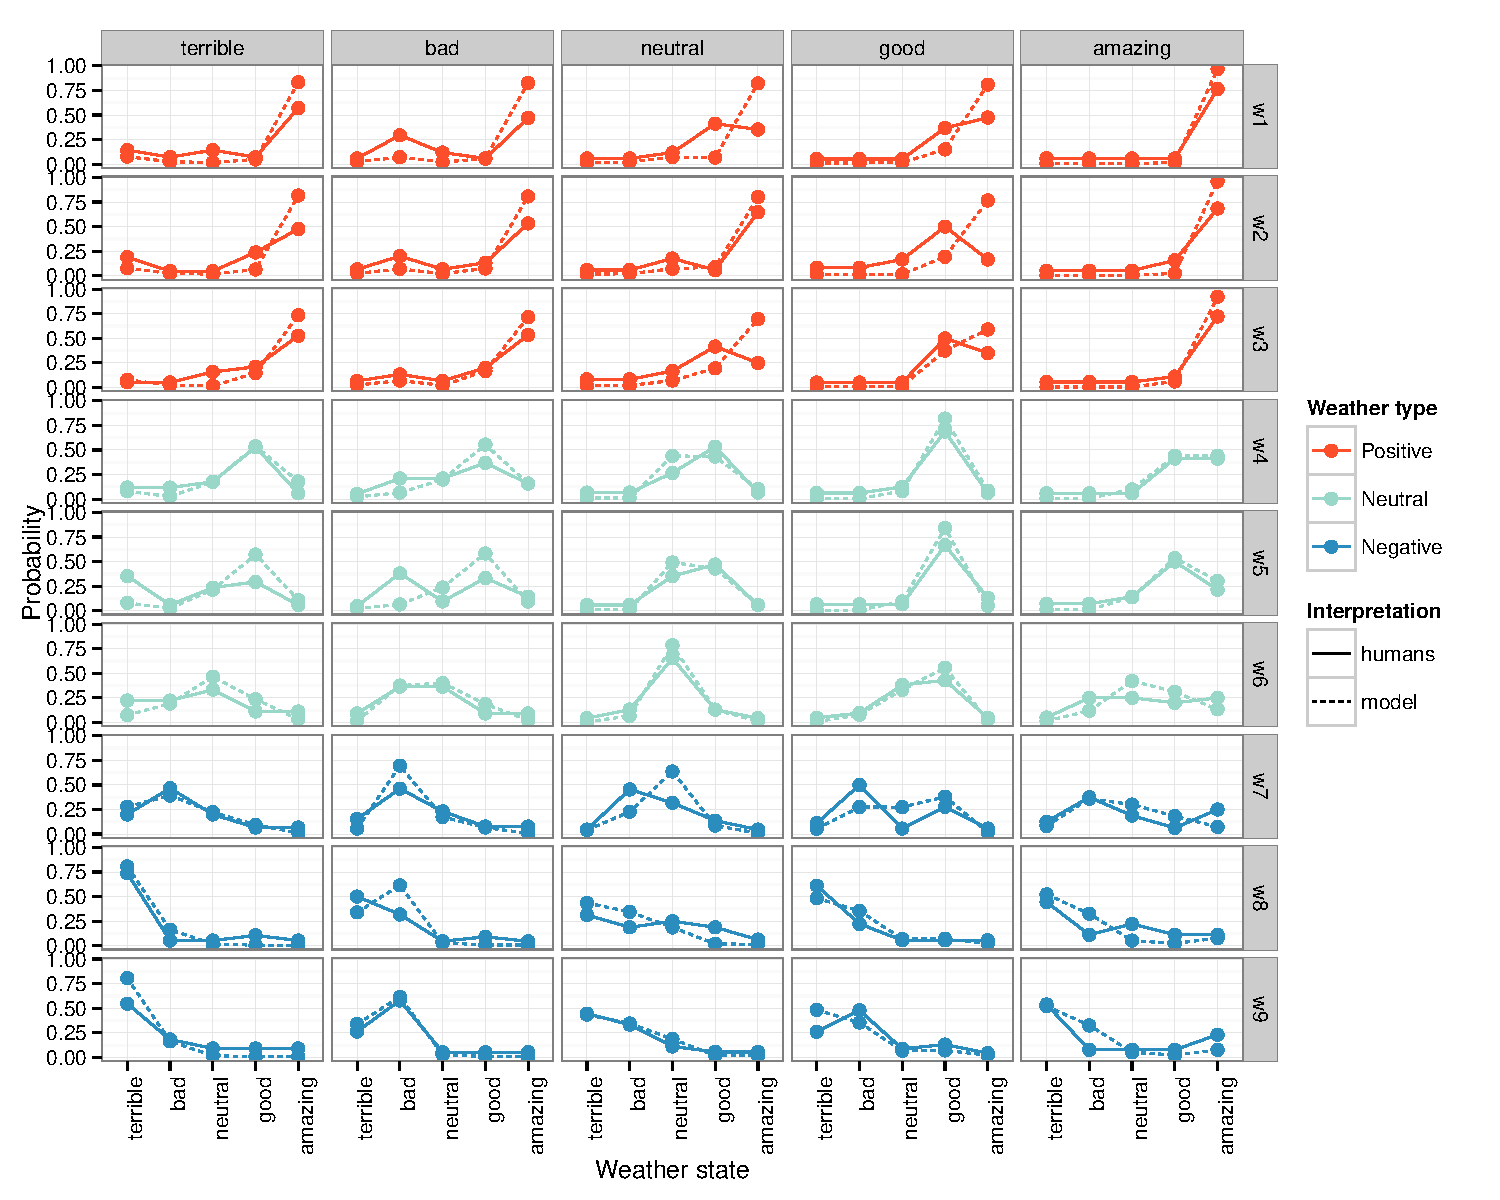
\includegraphics{model-state.pdf}}
\caption{Model's and participants' inferences about the weather state given a weather context and an utterance. Each panel represents an utterance about a weather context. The x axis are weather states. The light blue lines represent the model's distribution over weather states given an utterance about a weather context. The dark blue lines represent participants' distribution over weather states given an utterance about a weather context.}
\label{model-state}
\end{figure}

\section{Discussion}
\todo[inline]{summary of take-home point}
With our behavioral experiments, we presented results showing the fine-grained effects of background knowledge on people's interpretations of ironic utterances, and identified the main affective dimensions that are conveyed by irony. In addition, we presented a computational model that predicts peoples' interpretations of ironic utterances using general communicative principles. In effect, the model is able to tell when an utterance is meant to be literal or ironic, and when meant to be ironic, what types of affect the speaker intends to convey. By reasoning about the speaker's communicative goals, the model goes beyond the literal meaning of an utterance to infer the actual state of the world. In addition, it recovers important aspects of the speaker's affect about the situation and captures the social and affective uses of irony. Together, these results suggest that basic principles of communication---background knowledge and reasoning about informativeness with respect to the speaker's communicative goals---may be an important driver of irony understanding.

\todo[inline]{the above paragraph is murky. the below maybe gets more at our take-away point: the approach in kao2914 extends immediately to additional non-literal uses, by more carefully considering the space of covert meanings that may be conveyed. in general re-work this conclusion to be sharper, and clearer about the main points.}

\todo[inline]{connection to informal theories}

Since Grice's original proposal, there have been two competing theories of irony understanding. The echoic mention theory \cite{sperber1981irony, jorgensen1984test} proposes that ironic utterances are intended to remind the listener of a previous utterance that turned out to be false or irrelevant. The affective subtext of irony then arises from the contrast between what was said earlier and what is actually the case. On the other hand, pretense theory \cite{clark1984pretense} argues that when a speaker produces an ironic utterance, she is not genuinely making the utterance, but only pretending to be someone who would make such an utterance. Understanding an ironic statement then involves recognizing the pretense as well as the preposterousness of the person being enacted. (could make this whole part shorter) 

\todo[inline]{connection to NLP}
Given the prevalence of irony in natural language, many researchers in natural language processing aim to automatically detect sarcasm in large bodies of texts in order to recover the correct sentiment from an ostensibly positive or negative utterance (e.g. ``I was overjoyed to pay $\$30$ for an overcooked steak") \cite{davidov2010semi, filatova2012irony}. A critical insight that emerges from these approaches is that irony detection requires information far beyond surface linguistic cues, often calling upon a deep understanding of context and common knowledge between speaker and listener, which computers currently lack. Indeed, without sufficient contextual information, even human beings exhibit poor judgment of verbal irony \cite{gonzalez2011identifying, wallacehumans}.

\todo[inline]{relationship to hyperbole and what that says about figurative language understanding more generally}
It is important to note that the model we present here is only minimally different from the hyperbole model described earlier in the paper \cite{kao2014nonliteral}. In fact, the only difference is that instead of considering a single affect dimension (negative valence), this extended model takes seriously the circumplex model of affect (cite), which identifies valence and arousal as two main dimensions underlying the slew of emotions people experience. The similarities between these two models suggests that hyperbole and irony may be understood using similar principles of communication. A deeper point we wish to make with this work is that communication in general, and nonliteral language understanding in particular, relies on reasoning about the speaker's communicative goals during interpretation. Furthermore, these goals are often social or affective in nature, and speakers are adept at harnessing shared background knowledge with the listener to convey rich affective meanings without explicitly stating them. 

\todo[inline]{future directions and conclusion}
Our experimental paradigm and modeling framework lends itself well to a more detailed and precise account of irony understanding. For example, what are the range of social and affective meanings involved in irony understanding? We identified emotional valence and arousal in these experiments, but there may be others ....(attitudes? opinions? affect? social closeness?)
(TODO: finish) What are the social functions of irony? Irony is often used to signal social closeness with the listener, presumably because it expresses the speaker's assumption that she and the listener share a great deal of common ground (cite). Given an ambiguous utterance that could be interpreted either literally or ironically, if a speaker supplements the utterance with prosodic cues to signal that it is meant ironically, will listeners judge the speaker as being closer to them? Can our model more directly  test the predictions of the echoic mention and pretense theories of irony and help distinguish between them? Given the prevalence of irony in everyday language, we believe it would be \emph{amazing} (literally) to address these questions in future research and understand irony's mysterious ability to be interpreted as the opposite of what it is.

\todo[inline]{RDH: AMAZING discussion (but seriously, I think all the pieces are here, and you make a lot of neat connections). Overall, I'm wondering if there's a way to reduce the number of figures? 8 figures seems like a lot for a 6 page paper, and I'm worried you won't have space, especially if you want to add more figures for the results and model evaluation section (I counted three ``Figure XX'' placeholders). I didn't get much from 6 and 7, but maybe I just didn't understand the result they were showing. And maybe Figure 4 isn't needed, since it depicts the usual `valence/arousal' PCA space? Fig 1 and 2 could be combined into a multicolumn fig... }

\bibliographystyle{apacite}

\setlength{\bibleftmargin}{.125in}
\setlength{\bibindent}{-\bibleftmargin}

\bibliography{irony}


\end{document}
